%http://www.math.uconn.edu/~kconrad/blurbs/
\documentclass[oneside,a4paper,12pt]{article}
\usepackage[english,brazilian]{babel}
\usepackage[alf]{abntex2cite}
\usepackage[utf8]{inputenc}
\usepackage[T1]{fontenc}
\usepackage[top=20mm, bottom=20mm, left=20mm, right=20mm]{geometry}
\usepackage{framed}
\usepackage{booktabs}
\usepackage{color}
\usepackage{hyperref}
\usepackage{graphicx}
\usepackage{float}
\usepackage{pstricks}
\graphicspath{{./Figuras/}}    
\definecolor{shadecolor}{rgb}{0.8,0.8,0.8}
\usepackage{textcomp}
\usepackage{tikz}
\usepackage[utf8]{inputenc}
\usepackage{mathtext}
\usepackage{graphicx}
\usepackage{verbatim}
\usepackage{wrapfig}
\usepackage[T1]{fontenc}
\usepackage{blindtext}
\usepackage{tasks}
\usepackage{fancybox}
\usepackage{amsthm}
\usepackage{setspace}
\usepackage{amsmath}
\usepackage{amsfonts}
\usepackage{amssymb}
\usepackage{graphicx, color}
\newcommand{\under}{\texttt{\char`_}}
\newcommand{\sen}{{\rm sen}}
\newcommand{\tg}{{\rm tg}}
\newcommand{\cotg}{{\rm cotg}}
\newcommand{\cossec}{{\rm cossec}}
\newcommand{\arctg}{{\rm arctg}}
\newcommand{\arcsen}{{\rm arcsen}}
\newcommand{\negrito}[1]{\mbox{\boldmath{$#1$}}} 
\usepackage{pifont}
\usepackage{multicol}
\usepackage[framemethod=TikZ]{mdframed}
\newcommand{\heart}{\ensuremath\heartsuit}
\newcommand{\diamonde}{\ensuremath\diamondsuit}
\theoremstyle{Colorido}
\newtheorem{questao}{\textcolor{Floresta}{\textit{\bf Questão}}}
\newtheoremstyle{Colorido}{}{}{\color{Floresta}}{}{\color{Floresta}\bfseries}{}{ }{}
\newtheorem{theorem}{Theorem}
\newtheoremstyle{solu}{}{}{}{}{\color{red}\bfseries}{}{ }{}
\theoremstyle{solu}
\newtheorem*{resp}{Solução}
\newtheoremstyle{dotlessP}{}{}{}{}{\color{Floresta}\bfseries}{}{ }{}
\theoremstyle{dotlessP}
\newcommand{\solucao}[1]{\textcolor{blue}{\textbf{Solução:} #1}}
\newtheorem{sol}{Questão}
%FAZ EDICOES AQUI (somente no conteudo que esta entre entre as ultimas  chaves de cada linha!!!)
\newcommand{\universidade}{Programa de Iniciação Científica OBMEP}
\newcommand{\centro}{PIC 2020}
%\newcommand{\departamento}{Departamento}
%\newcommand{\curso}{Curso}
\newcommand{\professor}{Douglas de Araujo Smigly}
\newcommand{\disciplina}{Programa de Iniciação Científica}
\newcommand{\entrega}{ }
\DeclareSymbolFont{extraup}{U}{zavm}{m}{n}
\DeclareMathSymbol{\varheart}{\mathalpha}{extraup}{86}
\DeclareMathSymbol{\vardiamond}{\mathalpha}{extraup}{87}
	\cornersize{.3} 
	\mdfdefinestyle{MyFrame}{%
    linecolor=blue,
    outerlinewidth=2pt,
    roundcorner=20pt,
    innertopmargin=\baselineskip,
    innerbottommargin=\baselineskip,
    innerrightmargin=20pt,
    innerleftmargin=20pt,
    backgroundcolor=gray!24!white}
%ATE AQUI !!!

\begin{document}
\definecolor{Floresta}{rgb}{0.13,0.54,0.13}
	\pagestyle{empty}
	
	\begin{center}
	
\includegraphics[width=\linewidth/3]{logo_pic}%LOGOTIPO DA INSTITUICAO
	 	\vspace{0pt}
	 	
		\universidade
		\par
		\centro
		\par
%		\departamento
		\par
%		\curso
		\par
		\vspace{24pt}
		\LARGE \textbf{Avalia\c c\~ao - Ciclo III}
		
	\end{center}
	
	\vspace{24pt}
	
	%
%	\begin{tabular}{ |l|p{12cm}| }
%		
%		\hline
%		\multicolumn{2}{|c|}{\textbf{Dados de Identificação}} \\
%			\hline
%		Disciplina:        &    \disciplina          \\
%		\hline
%		Professor:         &    \professor           \\
%	\hline
%	Aluno(a):         &\\
%		\hline
%	Multiplicidade:  & \ \ \ \ \ \ \vline Nível: \vline\\
%	
%		\hline
	%\end{tabular}
	%
	

	\begin{tabular}{ |l|p{12cm}| }
		
		\hline
		\multicolumn{2}{|c|}{\textbf{Dados de Identificação}} \\
			\hline
		Curso:        &  \disciplina \\
			\hline
		Nome:        &  \\
		\hline
		Nível:      &  \\
		\hline
				Multiplicidade:      &  \\
		\hline
				Assinatura:      &  \\
		\hline
				Data de entrega:      &  \entrega \\
		\hline
	\end{tabular}
	
	\vspace{24pt}
	\vspace{40pt}
	\tableofcontents
	\begin{comment}	
\begin{multicols*}{2}
	\begin{center}
		\begin{tabular}{ |c|p{1.9cm}| }
		
		\hline
		\multicolumn{2}{|c|}{\textbf{Tarefa Online}} \\
			\hline
		\centering\textbf{Questão}        &  \textbf{Resposta}\\
		\hline
		Questão 1        & (b)\\
		\hline
		Questão 2        & (c)\\
		\hline
		Questão 3        & (c)\\
		\hline
		Questão 4        &\\
		\hline
		Questão 5        &\\
		\hline
		Questão 6        &\\
		\hline
		\textbf{Total}        &\\
		\hline
	\end{tabular}
	\end{center}
\columnbreak
		\begin{center}
		\begin{tabular}{ |c|p{1.9cm}| }
		
		\hline
		\multicolumn{2}{|c|}{\textbf{Avaliação Online}} \\
			\hline
		\centering\textbf{Questão}        &  \textbf{Resposta}\\
		\hline
		Questão 1        &\\
		\hline
		Questão 2        &\\
		\hline

		\textbf{Total}        &\\
		\hline
	\end{tabular}
	\end{center}
	
	\end{multicols*}
	\vspace{24pt}
	\end{comment}
	%\begin{snugshade}
	%	\section{O... aumento  }  
	%\end{snugshade}
	\newpage	
	\textcolor{Floresta}{\section{Tarefa Online}}
	\begin{sol}
\textit{(0,5 ponto)} \newline\newline
Um triângulo $ABC$ é retângulo com ângulo reto no vértice $A$. Seja $D$ o ponto de interseção da bissetriz interna de $ABC$ relativa ao vértice $B$ com o lado $AC$ de $ABC$. Se a distância de $D$ ao lado $BC$ de $ABC$ é igual a $5\mbox{ cm}$, então o comprimento do segmento de reta $AD$, em cm, é igual a:
\begin{tasks}[counter-format={(tsk[a])},label-width=3.6ex, label-format = {\bfseries}, column-sep = {20pt}](5)
\task[\textcolor{blue}{$\negrito{(a)} $}] $5$
\task[\textcolor{blue}{$\negrito{(b)} $}] $5,5$ 
\task[\textcolor{blue}{$\negrito{(c)} $}] $6$
\task[\textcolor{blue}{$\negrito{(d)} $}] $6,5$
\task[\textcolor{blue}{$\negrito{(e)} $}] $7$
\end{tasks}
\end{sol}
\solucao{Desenhemos uma figura para ilustrar o problema, sendo $E$ o ponto de interseção do segmento perpendicular a $BC$ com vértice em $D$:}
\begin{center}
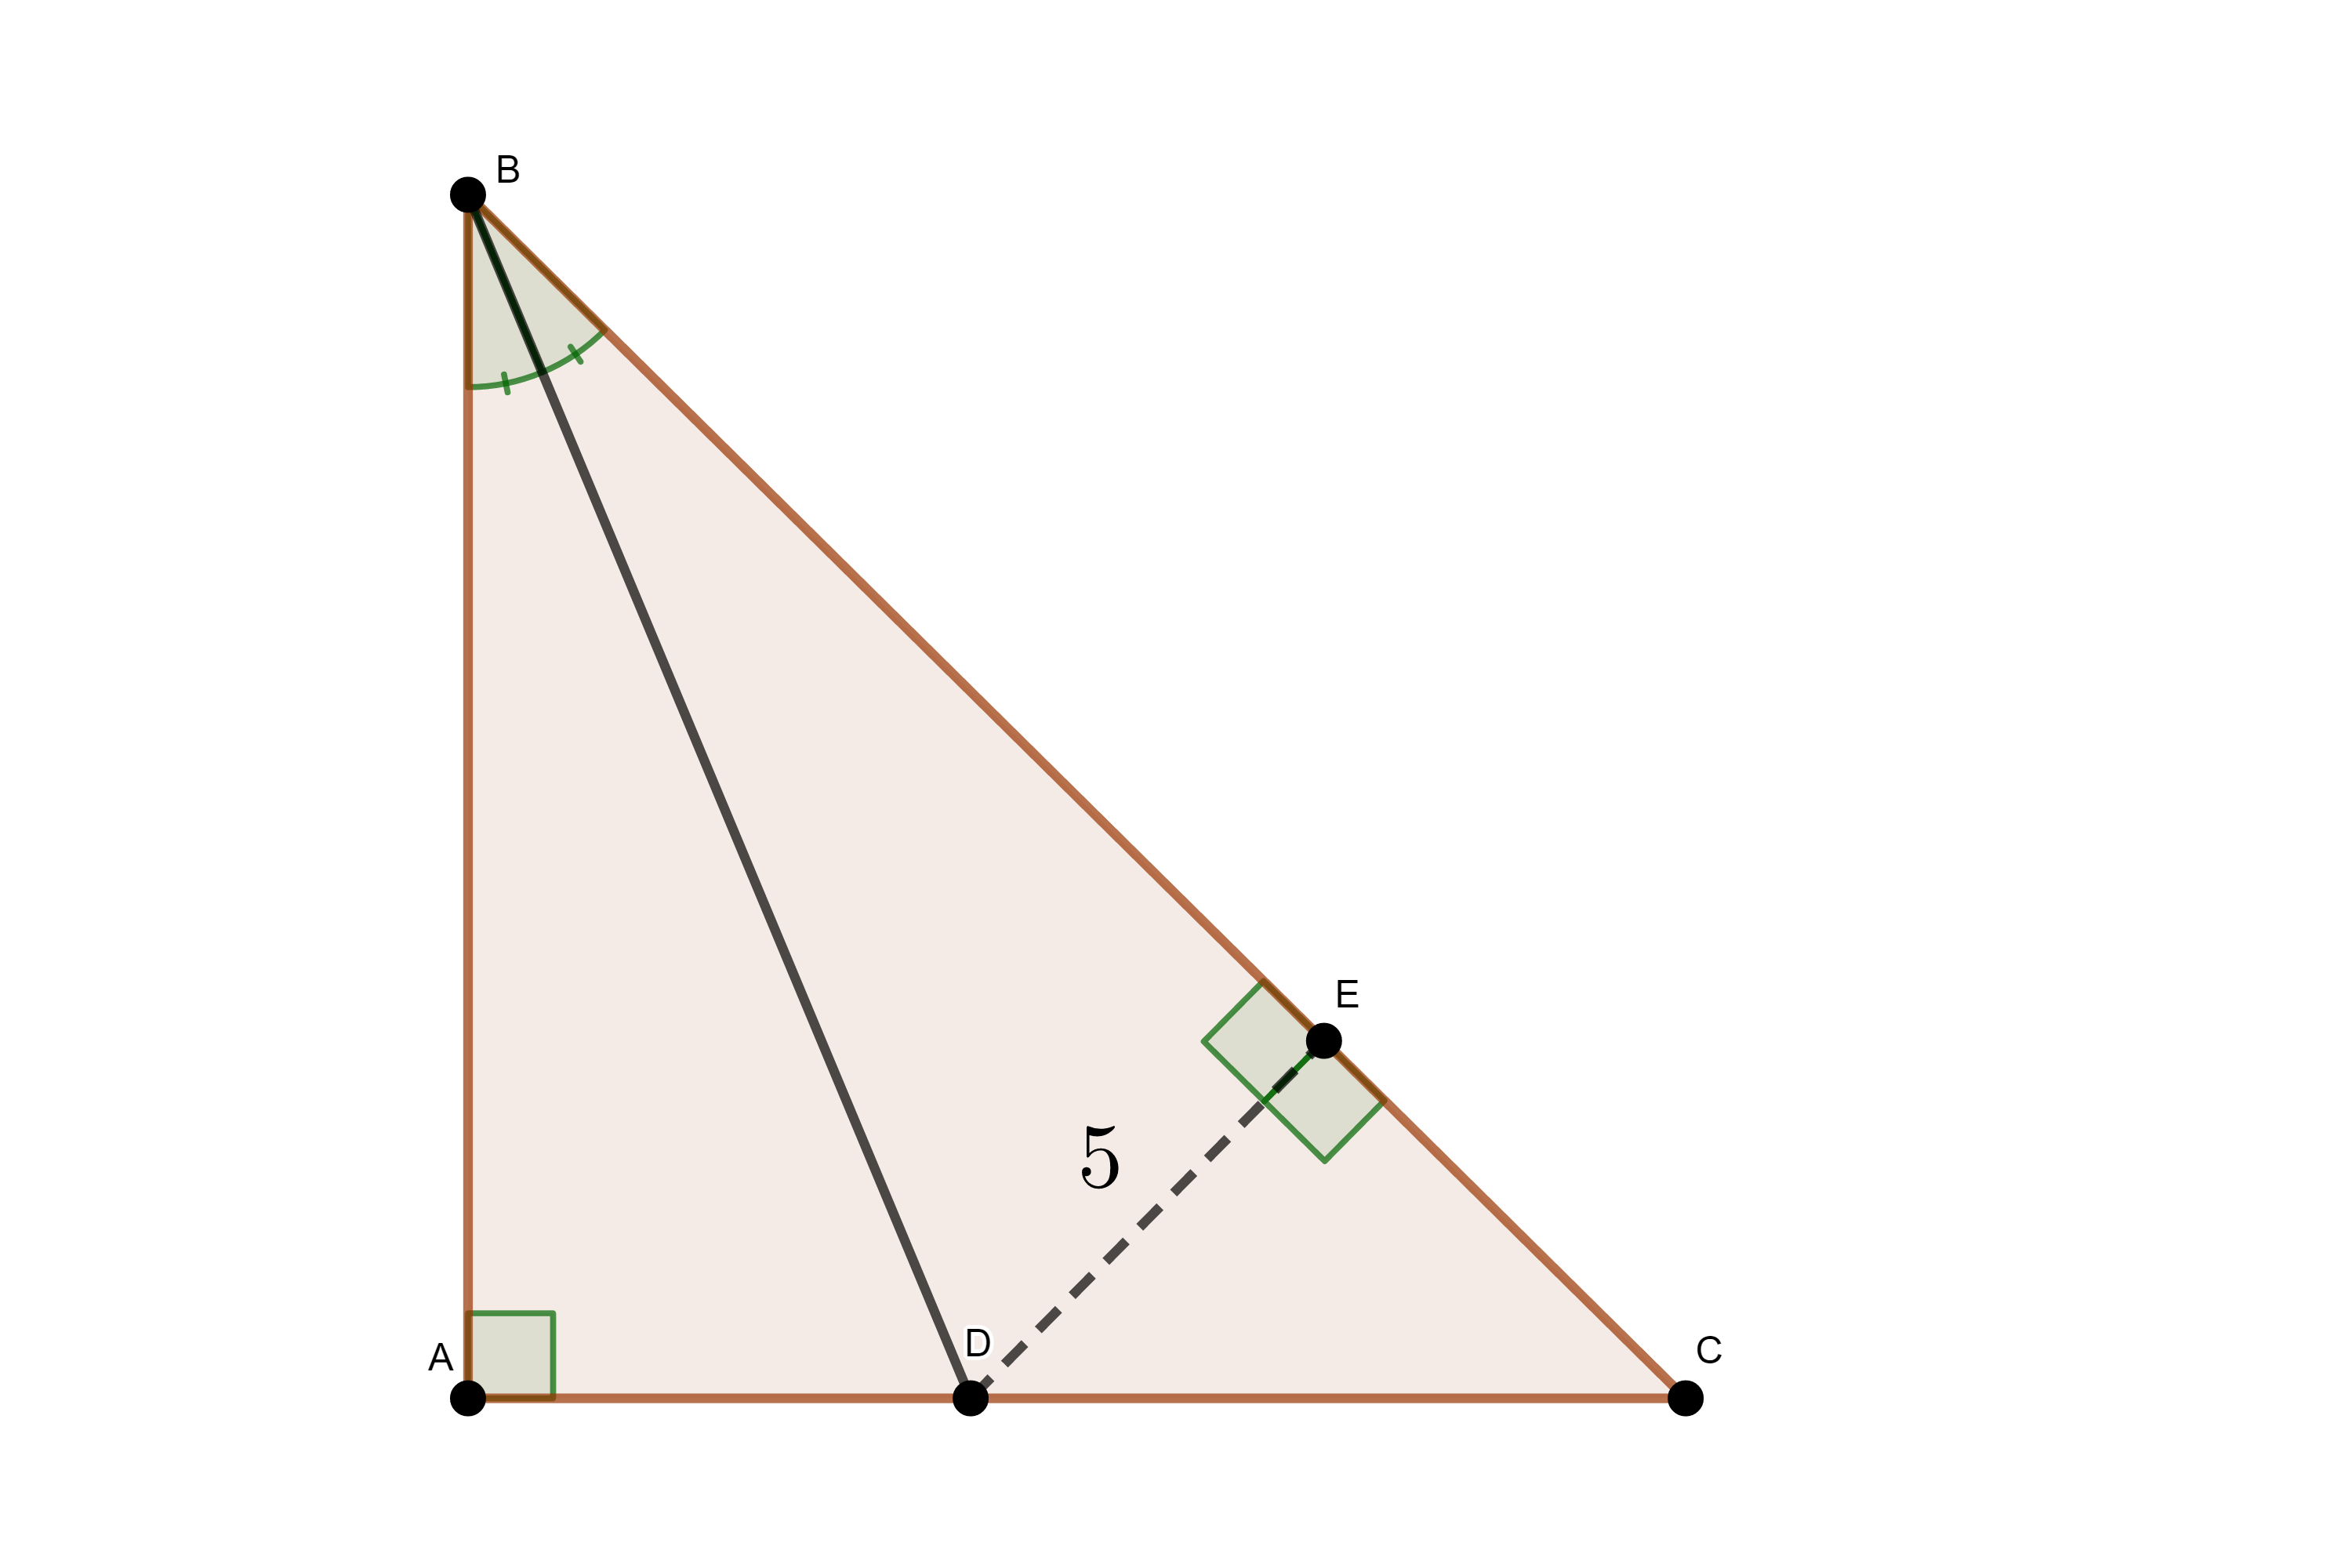
\includegraphics[scale=0.5]{Provas e Avaliações/Figuras avaliações/1avaliacaociclo3.png}
\end{center}
\textcolor{blue}{Pelo enunciado, temos que $DE = 5\mbox{ cm}.$ Além disso, como $BD$ é bissetriz interna de $\widehat{ABC},$ então $\widehat{ABD} = \widehat{DBE}.$ Observe também que $\widehat{BAD} = \widehat{BED} = 90^\circ.$ Dessa forma, como a soma dos ângulos internos de um triângulo é $180^{\circ},$
\[
\widehat{BDA} = 180^{\circ} - \textcolor{red}{\widehat{BAD}} - \textcolor{green}{\widehat{ABD}} = 180^{\circ} - \textcolor{red}{\widehat{BED}} - \textcolor{green}{\widehat{DBE}} = \widehat{DBE} \Rightarrow \widehat{BDA} = \widehat{DBE}.
\]
Como $\widehat{ABD}=\widehat{DBE}$, $\widehat{ADB}=\widehat{BDE}$ e $BD$ é lado comum a ambos os triângulos $ABD$ e $BDE$, então, pelo Caso de Congruência ALA, os triângulos $BAD$ e $BED$ são congruentes e, portanto, $AD=DE=5\mbox{ cm}$.}
		%\vspace{60pt}
		\newpage	
	\begin{sol}
\textit{(0,5 ponto)} \newline \newline
Sejam $ABC$ um triângulo equilátero, $P$ o ponto do lado $AC$ de $ABC$ tal que $AC = 8\cdot AP$, $Q$ o ponto do lado $AB$ de $ABC$ tal que $PQ$ seja paralelo a $BC$ e $R$ o ponto do lado $BC$ de $ABC$ tal que $QR$ seja paralelo a $AC$. A razão $\dfrac{(PQR)}{(ABC)}$, onde $(\mathcal F)$ denota a área da figura plana $\mathcal F$, é igual a:
\begin{tasks}[counter-format={(tsk[a])},label-width=3.6ex, label-format = {\bfseries}, column-sep = {20pt}](5)
\task[\textcolor{blue}{$\negrito{(a)} $}] $\dfrac{1}{3}$
\task[\textcolor{blue}{$\negrito{(b)} $}] $\dfrac{6}{7}$
\task[\textcolor{blue}{$\negrito{(c)} $}] $\dfrac{8}{75}$      
\task[\textcolor{blue}{$\negrito{(d)} $}] $\dfrac{7}{64}$
\task[\textcolor{blue}{$\negrito{(e)} $}] $\dfrac{5}{34}$
\end{tasks}
\end{sol}
\textcolor{blue}{\textbf{Solução:} Temos}
\begin{center}
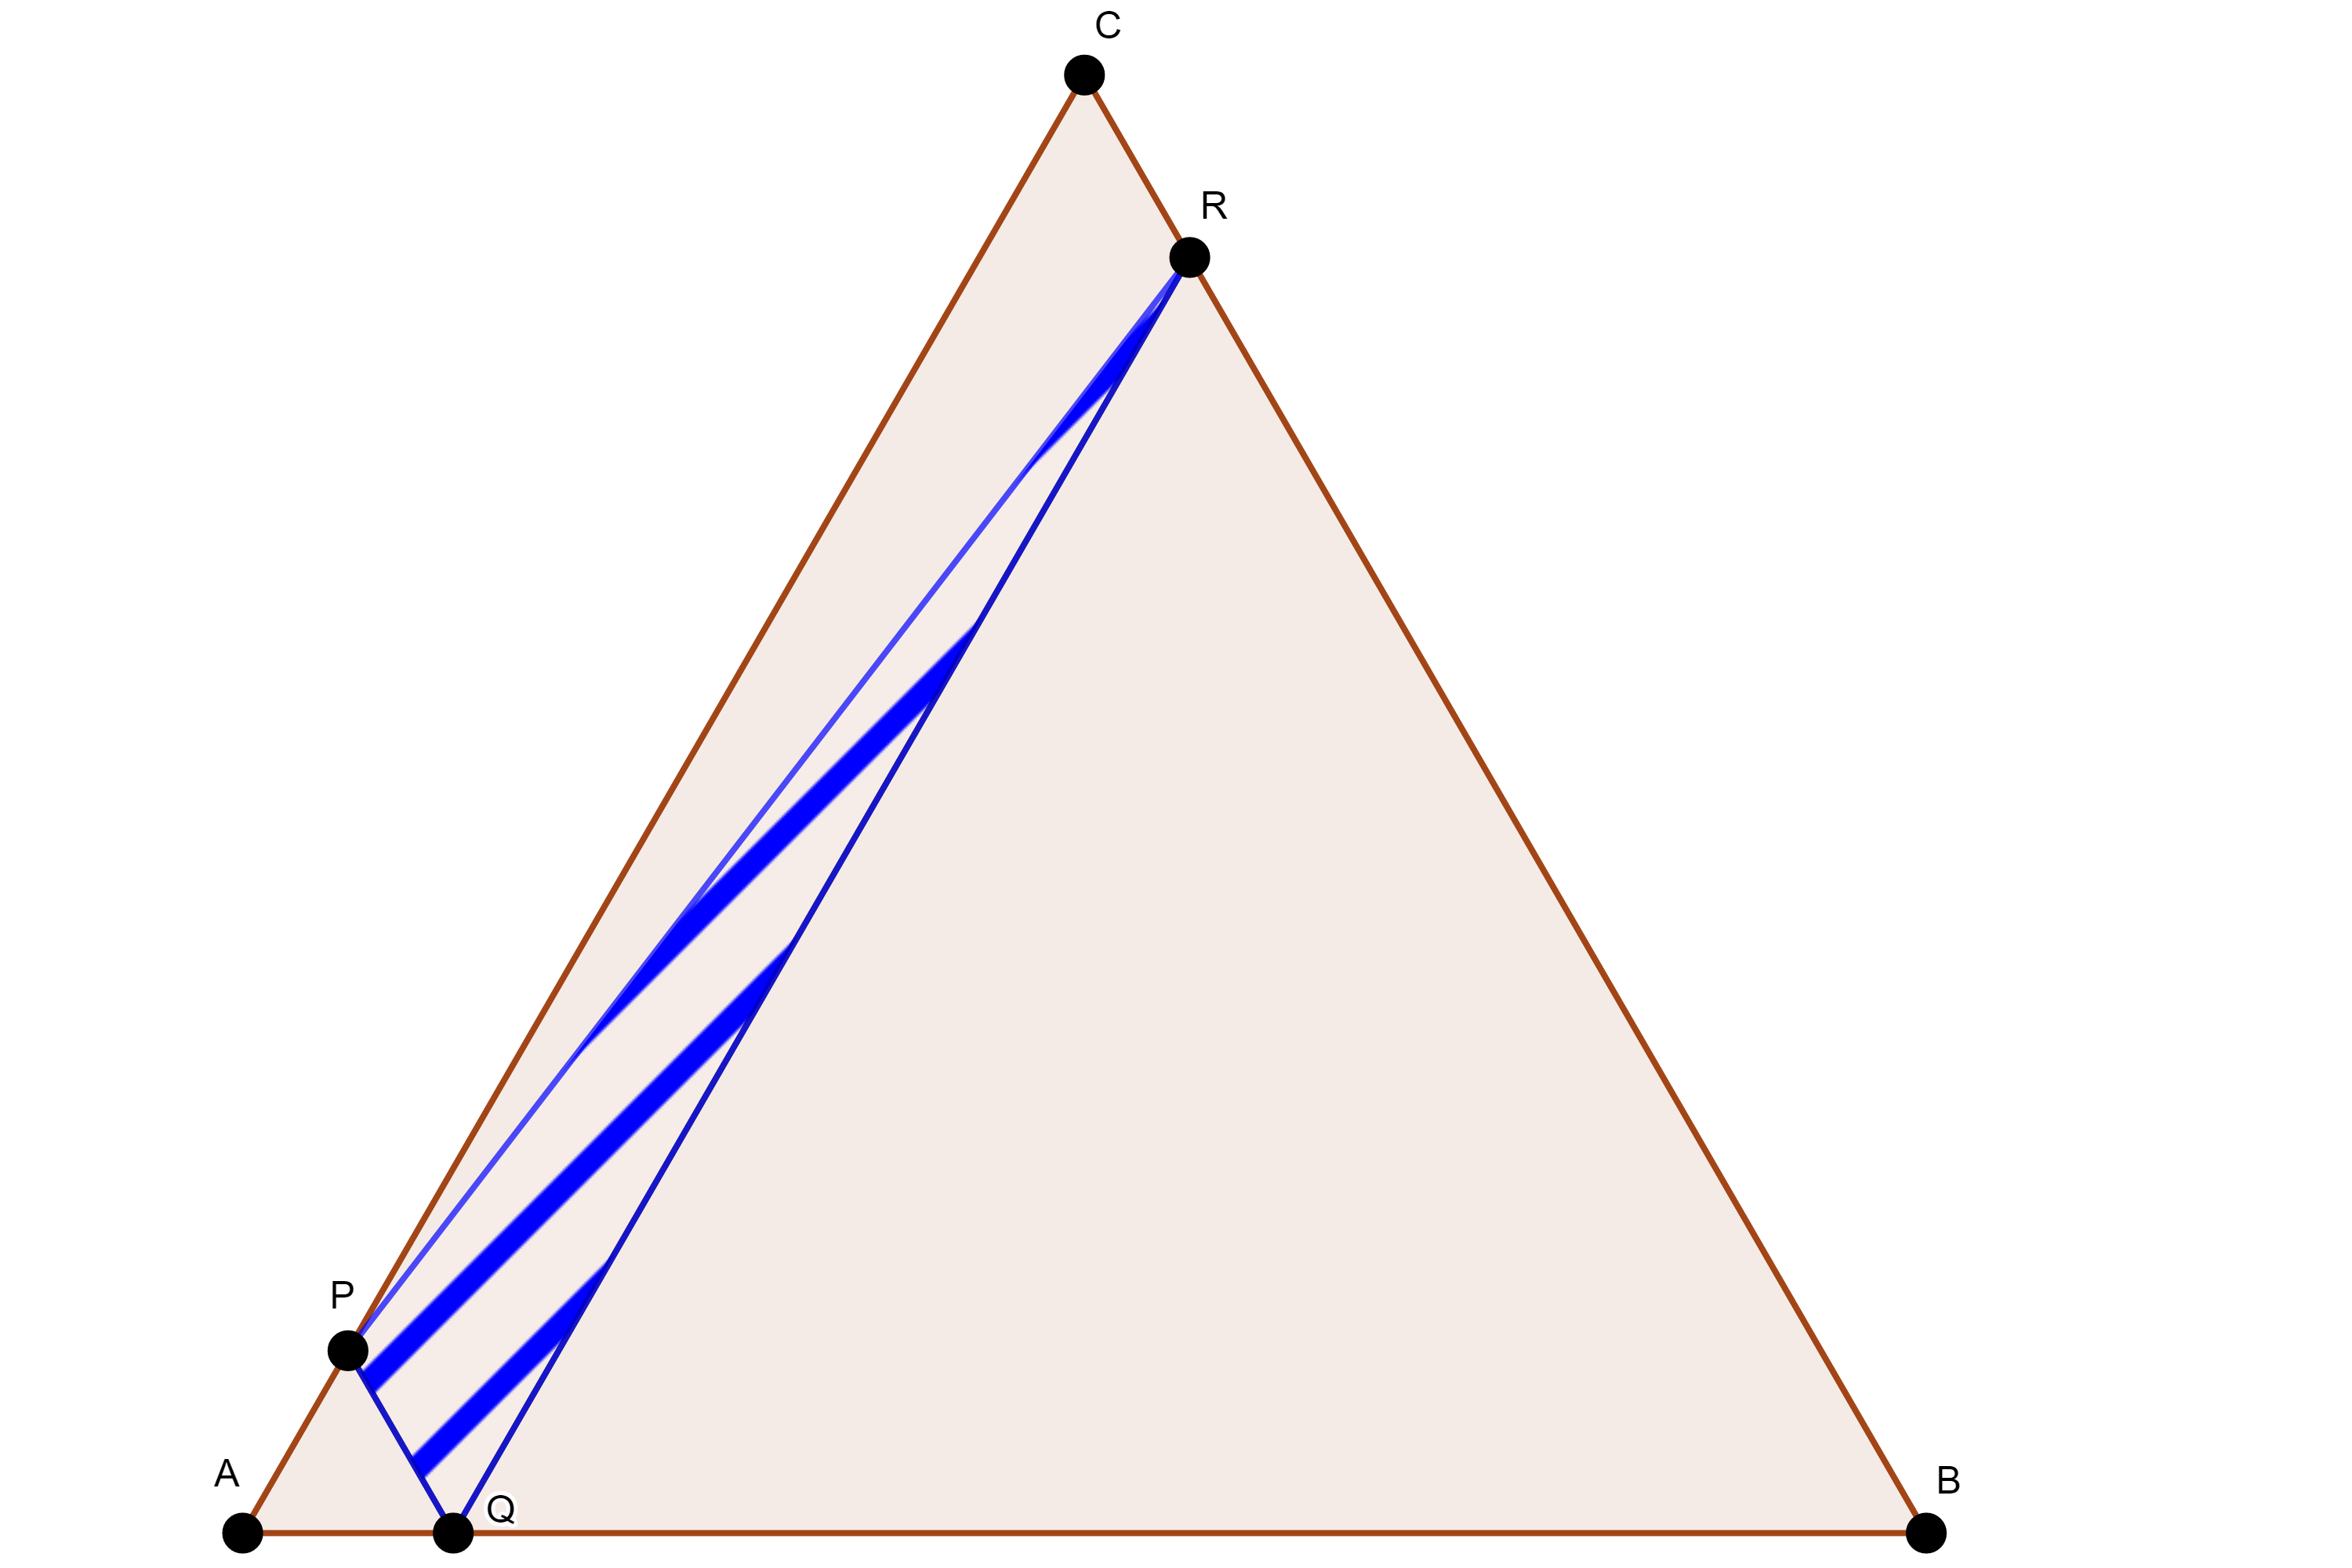
\includegraphics[scale=1.0]{Provas e Avaliações/Figuras avaliações/2avaliacaociclo3.png}
\end{center}
\textcolor{blue}{Como $PQ \parallel BC$ e $AC \parallel QR,$ os ângulos $\widehat{CPQ}$ e $\widehat{CRQ}$ são alternos internos, e portanto iguais. O mesmo ocorre com $\widehat{PCR}$ e $\widehat{PQR}.$ Assim, os ângulos dos triângulos $PCR$ e $PQR$ são iguais, e como ambos compartilham o lado $PR,$ pelo caso de congruência ALA, eles são congruentes. Novamente, pelo paralelismo de $PQ$ e $BC,$ $\widehat{APQ} = \widehat{ACB} = 60^\circ.$ Analogamente, $\widehat{PQA} = \widehat{CBA} = 60^\circ.$ Logo, $APQ$ é equilátero, bem como $QRB.$ Dado que $AP = AQ = \dfrac{1}{8} AC = \dfrac{1}{8} BC,$ temos que
\[\dfrac{(APQ)}{(ABC)} = \left( \dfrac{AP}{AC}  \right)^2 = \dfrac{1}{64} \quad \mbox{e} \quad \dfrac{(QRB)}{(ABC)} = \left( \dfrac{PC}{AC}  \right)^2 = \dfrac{49}{64}
\]
Portanto, 
\[\dfrac{(PQR)}{(ABC)} + \dfrac{(CPR)}{(ABC)} + \dfrac{(APQ)}{(ABC)} + \dfrac{(QRB)}{(ABC)} = 1 \Rightarrow 2\dfrac{(PQR)}{(ABC)} + \dfrac{1}{64} + \dfrac{49}{64} = 1 \Rightarrow \boxed{\dfrac{(CPR)}{(ABC)} = \dfrac{7}{64}}
\]}
\newpage
	\begin{sol}
\textit{(0,5 ponto)}  \newline\newline
Seja $ABC$ um triângulo retângulo isósceles ($AB=BC$), reto em $B$. Seja $D$ o ponto médio do segmento $BC$ e $\mathcal{C}$ a circunferência de centro $D$ e raio $BD$.
\begin{center}
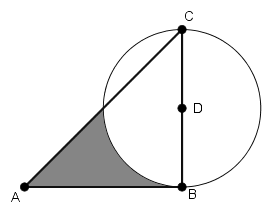
\includegraphics[scale=3.5]{Provas e Avaliações/Figuras avaliações/3avaliacaociclo3.png}
\end{center}
\begin{tasks}[counter-format={(tsk[a])},label-width=3.6ex, label-format = {\bfseries}, column-sep = {20pt}](5)
\task[\textcolor{blue}{$\negrito{(a)} $}] $\left(1 - \dfrac{\pi}{4} \right) R^2$
\task[\textcolor{blue}{$\negrito{(b)} $}] $\left(\dfrac{3}{2} - \dfrac{\pi}{4} \right) R^2$
\task[\textcolor{blue}{$\negrito{(c)} $}] $\left(2 - \dfrac{\pi}{2} \right) R^2$
\task[\textcolor{blue}{$\negrito{(d)} $}] $\left(2 - \dfrac{\pi}{4} \right) R^2$
\task[\textcolor{blue}{$\negrito{(e)} $}] $\left(3 - \dfrac{\pi}{2} \right) R^2$
\end{tasks}
\end{sol}
\solucao{Como $AB=BC$ e $R=BD=CD$, então $AB=BC=2R$. Assim, a área do triângulo $ABC$ é $\dfrac{2R \cdot 2R}{2}=2R^2$. Considere $E$ o ponto de interseção do segmento de reta $AC$ com a circunferência $\mathcal{C}$, como na figura:}
\begin{center}
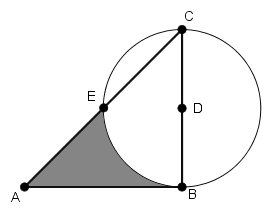
\includegraphics[scale=3.5]{Provas e Avaliações/Figuras avaliações/4avaliacaociclo3.png}
\end{center}

\textcolor{blue}{Como o triângulo $ABC$ é isósceles, reto em $B$, então $\widehat{ACB}=45^\circ$. Por outro lado, como $\widehat{ACB}=\dfrac{\widehat{EDB}}{2}$, então $\widehat{EDB} = 90^\circ$.\newline\newline Dessa forma, a área do triângulo $CDE$ é $\dfrac{R^2}{2}$ e a área do setor circular determinado pelo arco $BE$ é $\dfrac{\pi R^2}{4}$.\newline\newline Finalmente, a área hachurada é igual a $2R^2 - \dfrac{R^2}{2} - \dfrac{\pi R^2}{4} = \left(\dfrac{3}{2} - \dfrac{\pi}{4} \right) R^2$.}
\newpage
	\begin{sol}
\textit{(0,5 ponto)} \newline \newline Na figura abaixo, os pontos $B, C, D$ pertencem à circunferência de centro $A$. Sabendo que $\beta=\widehat{BCA}=15^\circ$ e $\gamma = \widehat{BDA}=25^\circ$, então a medida do ângulo $\alpha=\widehat{CAD}$ é:
\begin{center}
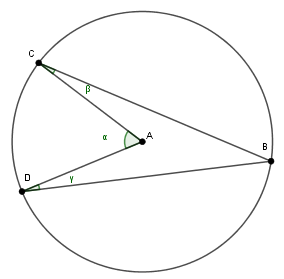
\includegraphics[scale=2.5]{Provas e Avaliações/Figuras avaliações/5avaliacaociclo3.png}
\end{center}

\begin{tasks}[counter-format={(tsk[a])},label-width=3.6ex, label-format = {\bfseries}, column-sep = {20pt}](5)
\task[\textcolor{blue}{$\negrito{(a)} $}] $40^\circ$
\task[\textcolor{blue}{$\negrito{(b)} $}] $50^\circ$
\task[\textcolor{blue}{$\negrito{(c)} $}] $60^\circ$
\task[\textcolor{blue}{$\negrito{(d)} $}] $70^\circ$
\task[\textcolor{blue}{$\negrito{(e)} $}] $80^\circ$
\end{tasks}
\end{sol}
\solucao{Trace o segmento $AB,$ como na figura:}
\begin{center}
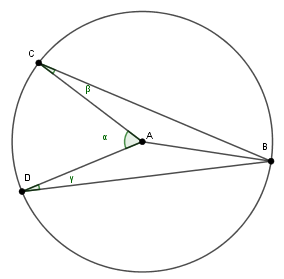
\includegraphics[scale=2.5]{Provas e Avaliações/Figuras avaliações/6avaliacaociclo3.png}
\end{center}
\textcolor{blue}{Veja que os triângulos $ABC$ e $ABD$ são isósceles, logo $\widehat{ABC}=\beta=15^\circ$ e $\widehat{ABD}= \gamma=25^\circ$. Como a soma dos ângulos internos de um triângulo é $180^\circ$ então $\widehat{BAC}=180^\circ - 2 \beta =150^\circ$ e $\widehat{BAD}= 180^\circ - 2 \gamma = 130^\circ$. Observe que $\alpha + \widehat{BAC} + \widehat{BAD}=360^\circ$ então $\alpha=360^\circ -150^\circ - 130^\circ=80^\circ$.}
\newpage
	\begin{sol}
\textit{(4 pontos)} \newline \newline
Na figura, $ABCD$ é um paralelogramo com triângulos equiláteros $ABE$ e $ADF$ construídos sobre os lados $AB$ e $AD$ de $ABCD$, respectivamente. Mostre que o triângulo $CEF$ é equilátero.
\begin{center}
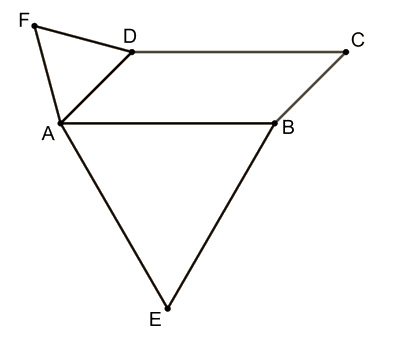
\includegraphics[scale=0.6]{Provas e Avaliações/Figuras avaliações/7avaliacaociclo3.png}
\end{center}
\end{sol}
\solucao{Para mostrar que $CEF$ é equilátero, basta verificar que $CE = CF = EF.$ }
\begin{center}
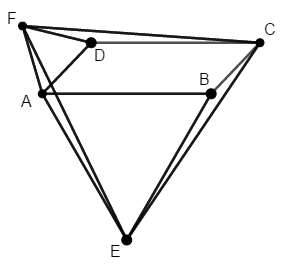
\includegraphics[scale=1.1]{Provas e Avaliações/Figuras avaliações/8avaliacaociclo3.png}
\end{center}
\textcolor{blue}{Para isso, é suficiente ver que $FDC, FAE$ e $EBC$ são triângulos congruentes. Sejam $\alpha = \widehat{DAB} = \widehat{DCB}$ e $\beta = \widehat{ADC} = \widehat{ABC}.$ Temos $\alpha + \beta = 90^\circ.$ Sendo $ABCD$ um paralelogramo e $ADF$ equilátero, $AD = BC = AF = FD.$ Analogamente, como $ABE$ é equilátero, $AB = AE = BE = CD.$
Calculemos agora os ângulos $\widehat{FDC}, \widehat{CBE}$ e $\widehat{FAE}:$
\[\begin{cases}
\widehat{FDC} = 360^\circ - \textcolor{red}{\widehat{FDA}} - \textcolor{green}{\widehat{ADC}} = 360^\circ  - \textcolor{red}{60^\circ} - \textcolor{green}{\beta} = 300^\circ - \beta \\
\widehat{EBC} = 360^\circ - \textcolor{red}{\widehat{ABE}} - \textcolor{green}{\widehat{ABC}} = 360^\circ  - \textcolor{red}{60^\circ} - \textcolor{green}{\beta} = 300^\circ - \beta\\
\widehat{FAE} = \textcolor{red}{\widehat{FAD}} + \textcolor{green}{\widehat{BAE}} + \textcolor{orange}{DAB} =  \textcolor{red}{60^\circ} + \textcolor{green}{60^\circ} + \textcolor{orange}{180^\circ - \beta} = 300^\circ - \beta
\end{cases}\]}
\begin{center}
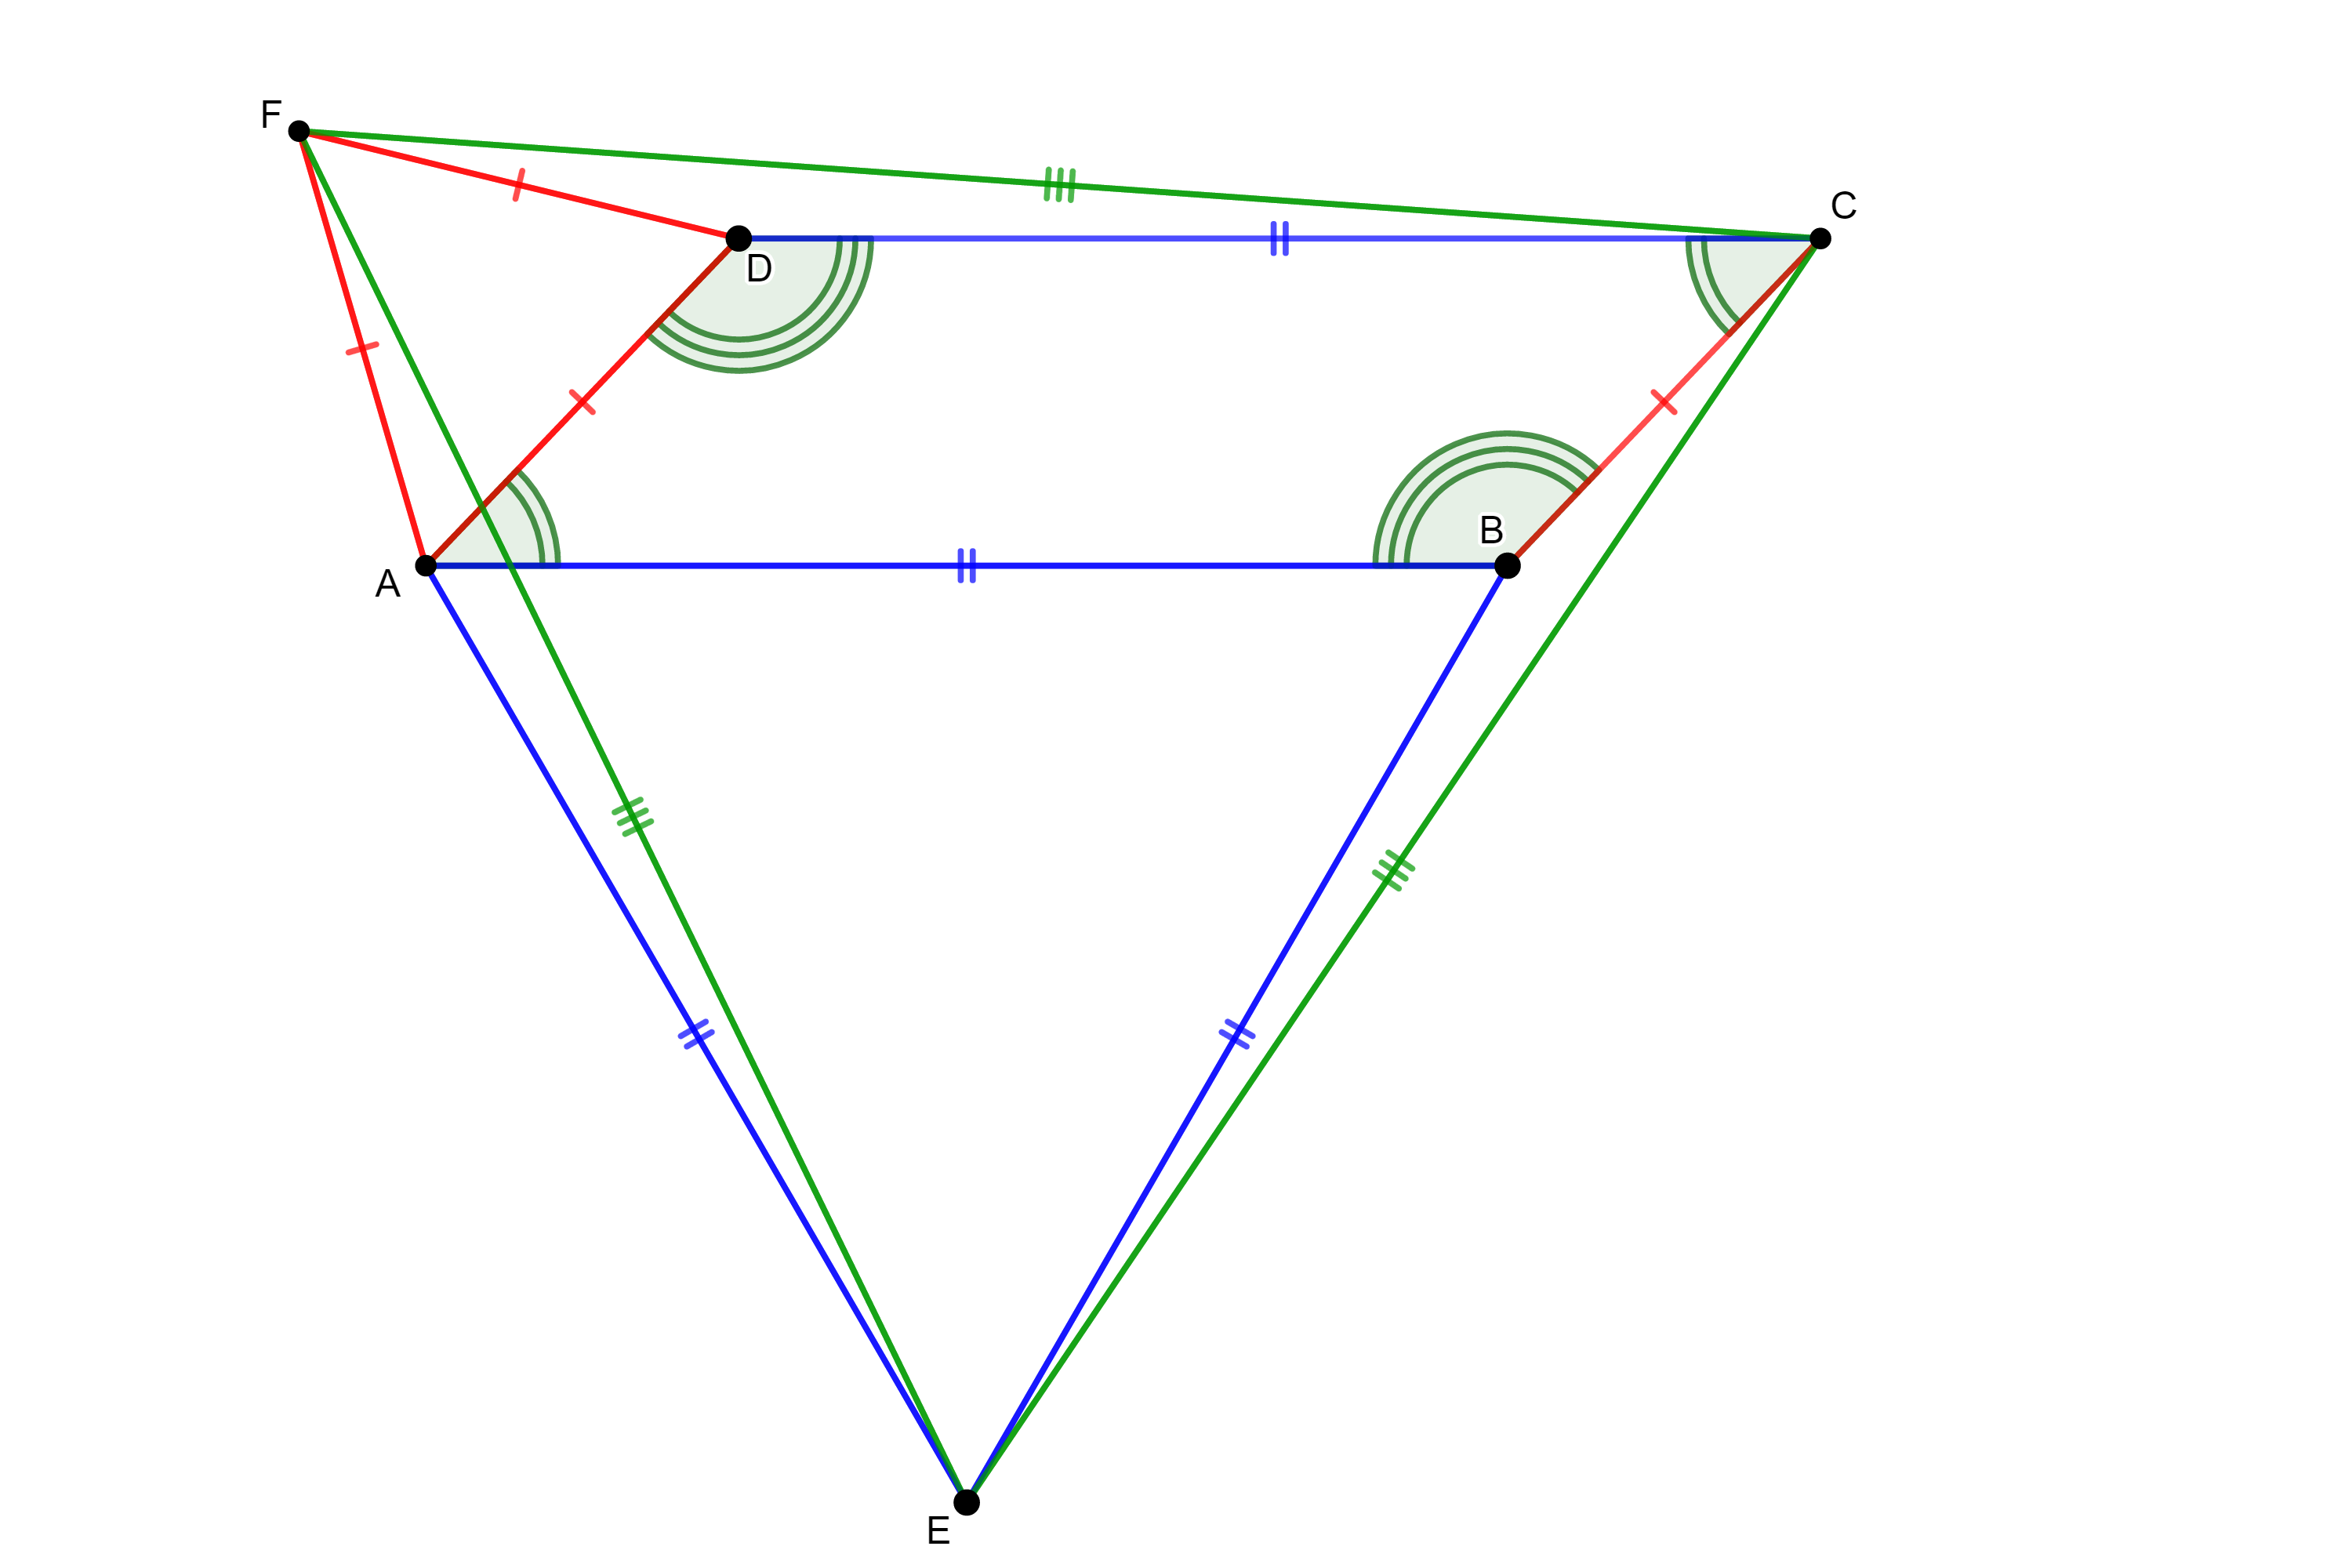
\includegraphics[scale=5.6]{Provas e Avaliações/Figuras avaliações/9avaliacaociclo3.png}
\end{center}
\textcolor{blue}{Assim, pelo caso de congruência LAL, $AEF,$ $DCF$ e $BEC$ são congruentes. Logo, $EF = CF = EC.$}
\newpage
	\begin{sol}
\textit{(4 pontos)} \newline \newline
Na figura abaixo, os pontos $A$, $B$, $C$, $D$, $E$, $F$, $G$ são centros das circunferências dadas, todas de mesmo raio $R=AB=BC=CD=DE=EF=FG=GB$.
\begin{center}
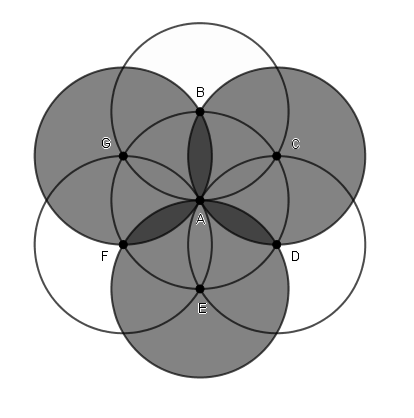
\includegraphics[scale=2.5]{Provas e Avaliações/Figuras avaliações/10avaliacaociclo3.png}
\end{center}
Observe também que os pontos $B,C,D,E,F,G$ se encontram sobre a circunferência de centro $A$ e raio $R$. Na figura, há uma região sombreada mais escura de área $\Gamma$ e uma região sombreada mais clara de área $\Omega$. Calcule $\Gamma$ e $\Omega$ em função de $R$.

\textsf{Dica:}  Use que a área de um triângulo equilátero de lado $L$ é igual a $\dfrac{\sqrt{3}}{4} L^2$,
\end{sol}
\solucao{Considere a figura formada unicamente por duas circunferências cuja interseção é uma parte da região mais escura, por exemplo, as circunferências de centros $E$ e $G$, como na figura abaixo.}
\begin{center}
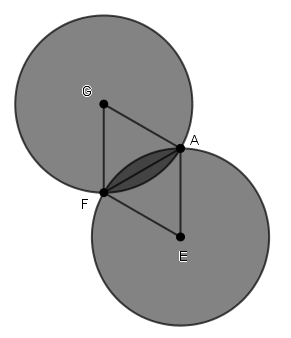
\includegraphics[scale=2.5]{Provas e Avaliações/Figuras avaliações/11avaliacaociclo3.png}
\end{center}
\textcolor{blue}{Seja $\Sigma$ a área da figura sombreada mais escura. Temos $\Gamma = 3 \Sigma$.\newline\newline Observe também que $AF=FG=GA$. Logo, o triângulo $AFG$ é equilátero e sua área é $\dfrac{\sqrt{3}}{4}R^2$. O ângulo em $G$ é $60^\circ$ e, portanto, a área do setor circular definido pelo ângulo $\widehat{AGF}$ na circunferência de centro $G$ é $\dfrac{\pi}{6}R^2$. Assim,\[\dfrac{1}{2}\Sigma = \dfrac{\pi}{6}R^2 - \dfrac{\sqrt{3}}{4}R^2 = \left(\dfrac{\pi}{6} -  \dfrac{\sqrt{3}}{4}\right) R^2 \Rightarrow \Sigma = \left(\dfrac{\pi}{3} -  \dfrac{\sqrt{3}}{2}\right) R^2.\] Dessa forma, $\Gamma = 3 \cdot \Sigma = \left(\pi -  \dfrac{3\sqrt{3}}{2}\right) R^2$.\newline\newline A área de uma circunferência é $\pi R^2$ e, na figura do enunciado, vemos que\[\Omega = 3 \left( \pi R^2 - 2 \Sigma  \right) = 3 \left( \pi  - 2 \left( \dfrac{\pi}{3} - \dfrac{\sqrt{3}}{2} \right)  \right) R^2= \left(\pi + 3\sqrt{3} \right)R^2.\]}
\newpage
	\textcolor{Floresta}{\section{Avaliação Online}}
	\begin{sol}
\textit{(5 pontos)} \newline \newline	
Na figura abaixo, os comprimentos dos segmentos de reta $CD$, $AE$ e $BF$ são iguais a um terço dos comprimentos dos lados $BC$, $AC$ e $AB$, respectivamente. É possível mostrar que $AG:GI:DI=3:3:1$, ou seja, os comprimentos dos segmentos de reta $AG$, $GI$ e $DI$ são diretamente proporcionais a $3$, $3$ e $1$, respectivamente; valendo o mesmo relativamente aos segmentos de reta $BE$ e $CF$.
\begin{center}
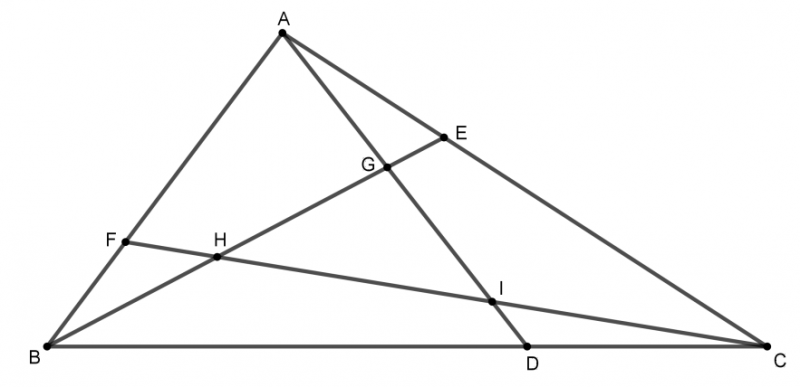
\includegraphics[scale=0.4]{Provas e Avaliações/Figuras avaliações/12avaliacaociclo3.png}
\end{center}
	\begin{tasks}[counter-format={(tsk[a])},label-width=3.6ex, label-format = {\bfseries}, column-sep = {20pt}](1)
\task[\textcolor{blue}{$\negrito{(a)} $}] Mostre que $(ACD)=\dfrac{1}{3}(ABC)$, sendo que $(\mathcal T)$ denota a área do triângulo $\mathcal T$. 

\task[\textcolor{blue}{$\negrito{(b)} $}] Mostre que $(CDI)=\dfrac{1}{21}(ABC)$.
\task[\textcolor{blue}{$\negrito{(c)} $}] Calcule a razão $\dfrac{(GHI)}{(ABC)}$.
\end{tasks}
\end{sol}
\solucao{\begin{tasks}[counter-format={(tsk[a])},label-width=3.6ex, label-format = {\bfseries}, column-sep = {20pt}](1)\task[\textcolor{blue}{$\negrito{(a)} $}] Observe que os triângulos $ABC$ e $ACD$ compartilham a mesma altura $h,$ e é fornecido no enunciado que $CD = \dfrac{BC}{3}.$ Logo,\[(ACD) = \dfrac{CD \cdot h}{2} = \dfrac{\dfrac{BC}{3} \cdot h}{2} = \dfrac{1}{3} \left( \dfrac{BC \cdot h}{2} \right) = \dfrac{1}{3}(ABC) \Rightarrow \boxed{(ACD) = \dfrac{1}{3}(ABC)} \]\end{tasks}}
\begin{center}
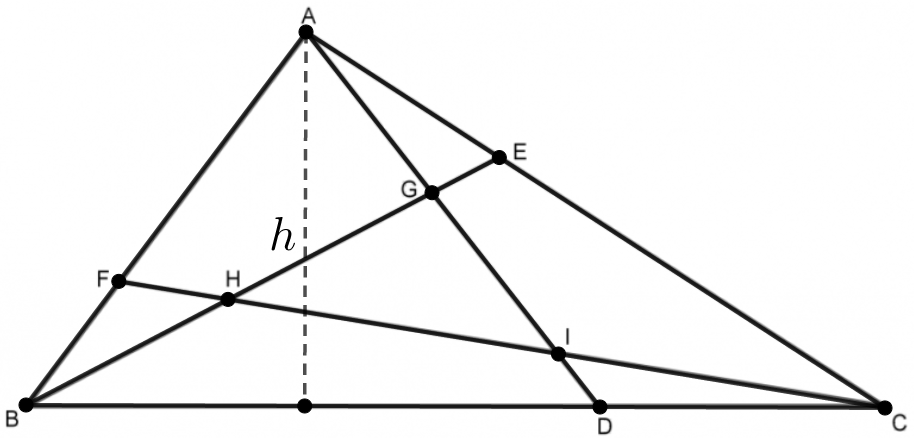
\includegraphics[scale=0.4]{Provas e Avaliações/Figuras avaliações/13avaliacaociclo3.png}
\end{center}
\textcolor{blue}{\begin{tasks}[counter-format={(tsk[a])},label-width=3.6ex, label-format = {\bfseries}, column-sep = {20pt}](1)
\task[\textcolor{blue}{$\negrito{(b)} $}] Seja  $h^\prime$ a altura do triângulo $CDI$ relativa ao vértice $I,$ como na figura:\end{tasks}}
\begin{center}
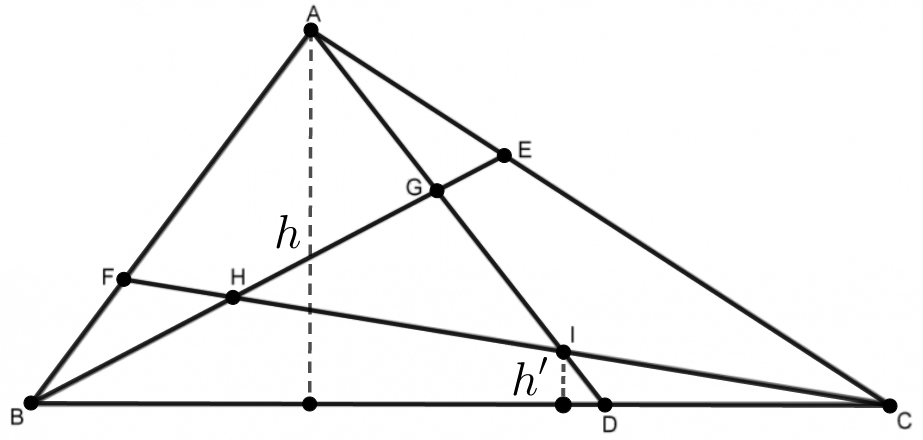
\includegraphics[scale=0.4]{Provas e Avaliações/Figuras avaliações/14avaliacaociclo3.png}
\end{center}
\textcolor{blue}{Como $AG:GI:DI=3:3:1,$ então \[\dfrac{DI}{AD} = \dfrac{1}{3 + 3 + 1} = \dfrac{1}{7}.\]
Como os triângulos $ADh$ e $IDh^\prime$ são semelhantes, temos que\[\dfrac{AD}{ID} = \dfrac{h}{h^\prime} \Rightarrow  \dfrac{AD}{\dfrac{AD}{7}} = \dfrac{h}{h^\prime}  \Rightarrow h^\prime = \dfrac{1}{7}h.\]
Assim,\[(CDI) = \dfrac{\textcolor{red}{DC}\cdot \textcolor{green}{h^{\prime}}}{2} = \dfrac{\textcolor{red}{\dfrac{1}{3}BC} \cdot \textcolor{green}{\dfrac{1}{7}h}}{2} = \dfrac{1}{21} \dfrac{BC \cdot h}{2} = \dfrac{1}{21} (ABC) \Rightarrow \boxed{(CDI) =\dfrac{1}{21} (ABC) }\]}
\textcolor{blue}{\begin{tasks}[counter-format={(tsk[a])},label-width=3.6ex, label-format = {\bfseries}, column-sep = {20pt}](1)
\task[\textcolor{blue}{$\negrito{(c)} $}] Observe que podemos decompor o triângulo $ABC$ em 4 triângulos, sendo eles $\textcolor{green}{ACI}, \textcolor{blue}{CBH},$ $\textcolor{red}{ABG}$ e $\textcolor{orange}{GHI},$ como mostrado na figura.
\end{tasks}}
\begin{center}
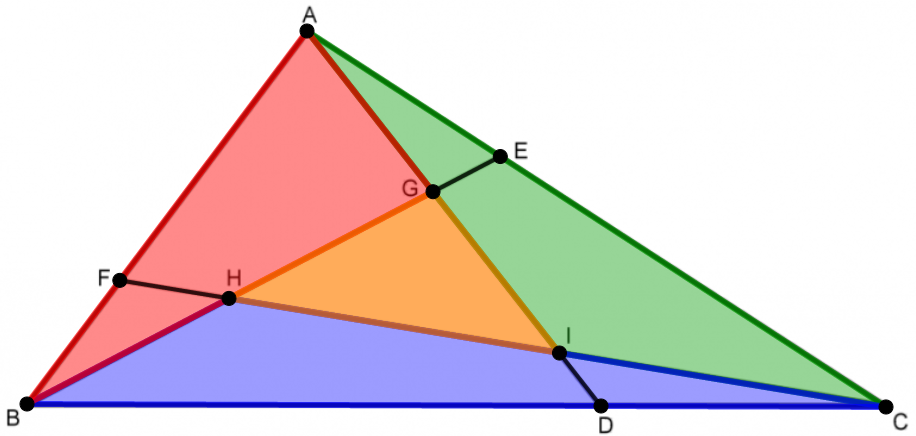
\includegraphics[scale=0.4]{Provas e Avaliações/Figuras avaliações/15avaliacaociclo3.png}
\end{center}
\textcolor{blue}{O que foi feito nos itens (a) e (b) em relação aos triângulos $CDI$ e $ACD$ pode ser reproduzido com os triângulos $BHF$ e $CBF$ e analogamente com $ABE$ e $AEG.$ Assim, temos que\[\begin{array}{ccc}(ADC) = \dfrac{1}{3}(ABC) & \mbox{e} & (CDI) = \dfrac{1}{3}(ABC)\\(CBF) = \dfrac{1}{3}(ABC) & \mbox{e} & (BHF) = \dfrac{1}{3}(ABC) \\(ABE) = \dfrac{1}{3}(ABC) & \mbox{e} & (AEG) = \dfrac{1}{3}(ABC)\\\end{array}\]Logo,\[\begin{array}{rcl}(ABC) &=& \textcolor{green}{(ACI)} + (CBH) + \textcolor{red}{(ABG)} + \textcolor{orange}{(GHI)} \Rightarrow \\
&=& \textcolor{green}{\left((ADC) - (CDI)\right)} + \left( (CBF) - (BHF)\right) + \textcolor{red}{\left( (ABE) - (AG) \right)} + \textcolor{orange}{(GHI)} \\ &=& \textcolor{green}{\left(\dfrac{1}{3}(ABC) - \dfrac{1}{21}(ABC)\right)} + \left(\dfrac{1}{3}(ABC) - \dfrac{1}{21}(ABC)\right) +\textcolor{red}{\left(\dfrac{1}{3}(ABC) - \dfrac{1}{21}(ABC)\right)}   \\
&\phantom{=}& + \textcolor{orange}{(GHI)} \\
&=& 3 \left( \dfrac{1}{3}(ABC) - \dfrac{1}{21}(ABC)\right) + (GHI) \\&=& \dfrac{6}{7}(ABC) + (GHI) \Rightarrow (GHI) = \dfrac{1}{7}(ABC).\end{array}\]
Portanto,\[\dfrac{(GHI)}{(ABC)} = \dfrac{\dfrac{1}{7}(ABC)}{(ABC)} = \dfrac{1}{7}.\] \newline \newline \textbf{Solução Alternativa:} Observe que $\dfrac{CE}{AE} = \dfrac{BD}{DC} = \dfrac{AF}{BF} = 2.$ Assim, aplicando o Teorema de Routh, temos que \[\dfrac{(GHI)}{(ABC)} = \dfrac{\left(\dfrac{CE}{AE} \cdot \dfrac{BD}{DC} \cdot \dfrac{AF}{BF} - 1\right)^2}{\left(\dfrac{CE}{AE}  \cdot \dfrac{BD}{DC} + \dfrac{BD}{DC} + 1\right)\left( \dfrac{BD}{DC} \cdot \dfrac{AF}{BF} + \dfrac{AF}{BF} + 1\right)\left(\dfrac{AF}{BF} \cdot \dfrac{CE}{AE}  + \dfrac{CE}{AE}  + 1\right)} = \]\[\dfrac{(2 \cdot 2 \cdot 2 - 1)^2}{(2 \cdot 2+ 2 + 1)(2 \cdot 2+ 2 + 1)(2 \cdot 2+ 2 + 1)} = \dfrac{7^2}{7^3} = \dfrac{1}{7}.\]}
\begin{mdframed}
\textbf{Critérios de Correção:} \\
\textbf{(a)} 
\begin{itemize}
    \item Atribuir $0,5$ ponto se o aluno observar que as alturas dos triângulos $ABC$ e $ACD$ relativas ao vértice $A$ são iguais.
    \item Atribuir $0,5$ ponto se o aluno observar que $CD=\dfrac{1}{3}BC$.
    \item Atribuir $0,5$ ponto se o aluno concluir corretamente que $(ACD)=\dfrac{1}{3}(ABC)$.
\end{itemize}
\textbf{(b)} 
\begin{itemize}
    \item Atribuir $0,5$ ponto se o aluno observar que as alturas dos triângulos $ACD$ e $CDI$ relativas ao vértice $C$ são iguais.
    \item Atribuir $0,5$ ponto se o aluno observar que $DI=\dfrac{1}{7}AD$.
    \item Atribuir $0,5$ ponto se o aluno concluir corretamente que $(CDI)=\dfrac{1}{21}(ABC)$.
\end{itemize}
\textbf{(c)} 
\begin{itemize}
    \item Atribuir $1,0$ ponto se o aluno expressar corretamente $(GHI)$ ou $(ABC)$ como soma e diferença de áreas de triângulos.
    \item Atribuir $1,0$ ponto se o aluno calcular corretamente a resposta final.
\end{itemize}
\end{mdframed}
\newpage
	\begin{sol}
\textit{(5 pontos)} \newline \newline
Circunscreve-se um círculo a um quadrado de lado $2\mbox{ cm}$. Sobre cada lado do quadrado, considera-se a semicircunferência exterior ao quadrado com centro no ponto médio do lado e raio $1\mbox{ cm}$, como na figura a seguir. Calcule a área da região hachurada.
\begin{center}
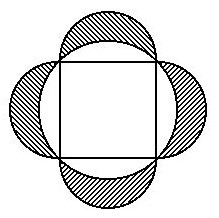
\includegraphics[scale=1.0]{Provas e Avaliações/Figuras avaliações/16avaliacaociclo3.png}
\end{center}
\end{sol}
\solucao{A figura abaixo representa a área limitada pelos semicírculos. Para calculá-la é preciso calcular a área do quadrado e somar com a área dos quatro semicírculos.}
\begin{center}
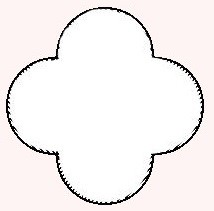
\includegraphics[scale=1.0]{Provas e Avaliações/Figuras avaliações/17avaliacaociclo3.png}
\end{center}
\textcolor{blue}{O lado do quadrado mede $2\mbox{ cm}$ e sua área é $A_q=2^2=4\mbox{ cm}^2$. Agora, basta calcular a área de um semicírculo e multiplicar por $4$ deles no exercício. A área de um semicírculo é $A_s=\dfrac{\pi\cdot1^2}{2}=\dfrac{\pi}{2}$. Assim, a área delimitada pelos semicírculos é \[A_c=A_q+4A_s=4+2\pi.\]A área da região hachurada é igual á área delimitada pelos semicírculos menos a área do círculo no qual o quadrado está inscrito. Resta então calcular o seu raio.\newline \newline Sejam $A$, $B$, $C$ e $D$ os vértices do quadrado e $M$ o ponto de interseção das diagonais (que é também o centro da circunferência onde o quadrado se encontra inscrito).}
\begin{center}
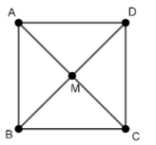
\includegraphics[scale=4]{Provas e Avaliações/Figuras avaliações/18avaliacaociclo3.png}
\end{center}
\textcolor{blue}{Como os triângulos retângulos $ABC$ e $ACD$ são isósceles, então os ângulos da figura que têm $M$ como vértice medem $90^\circ$. Chamando de $R$ o raio da circunferência de centro $M$ e raio $MA$, temos \[A_{ABCD}=A_{ABD}+A_{BCD}= 2 \left( \dfrac{2R \cdot 2R}{2} \right) = 2R^2\]Como a área do quadrado é $4$, então $R=\sqrt2$. Assim, a área do círculo de raio $R$ é $\pi R^2=2\pi$\newline \newline Finalmente, a área da região hachurada é $4+2\pi-2\pi=4\mbox{ cm}^2$.}
\begin{mdframed}
\textbf{Critérios de Correção:} \\
\begin{itemize}
    \item Atribuir $1,0$ ponto se o aluno calcula a área de um dos semicírculos.
    \item Atribuir $1,0$ ponto se o aluno calcula a área delimitada pelos semicírculos (a soma das áreas dos quatro semicírculos e a área do quadrado).
    \item Atribuir $1,0$ ponto se o aluno calcula a área do círculo no qual o quadrado está inscrito.
    \item Atribuir $1,0$ ponto se o aluno escreve que a área hachurada é igual à diferença entre a área delimitada pelos semicírculos e a área do círculo no qual o quadrado está inscrito.
    \item Atribuir $1,0$ ponto se o aluno calcula a área hachurada.
\end{itemize}
\end{mdframed}
		%\vspace{60pt}
%		\newpage
		%QUESTAO 2
		
		%\vspace{60pt}
	
		%QUESTAO 3

		%\vspace{60pt}
		
		%QUESTAO 4 (OBJETIVA)

		
		%a)(  ) Alternativa A.
		
	%	b)(  ) Alternativa B.
		
	%	c)(  ) Alternativa C.
		
	%	d)(  ) Alternativa D.
		
	\flushbottom
	\flushright
%	"Alguma frase bonita de fim de prova"\\(autor da frase bonita)
\end{document}
\begin{center}
\includegraphics[scale=0.48]{paralelepipedo_p1}
\end{center}
	\begin{sol}
\textit{(4 pontos)} \newline \newline
\end{sol}
\solucao{}
\newpage
